%! Author = Omar Iskandarani
%! Date = 2/15/2025
\documentclass[a4paper,10pt]{article}
\usepackage{amsmath, amssymb, graphicx, hyperref, physics}
\usepackage[a4paper,margin=1in]{geometry}
\usepackage{array}
\usepackage{booktabs}
\usepackage{amsmath, amssymb, graphicx, hyperref, physics}
\geometry{margin=1in}


\title{The Vortex \AE ther Model: A Vorticity-Based Framework for Gravity and Electromagnetism}
\author{Omar Iskandarani}
\date{\today}

\begin{document}
    \maketitle

    \maketitle

    \begin{abstract}
        This paper introduces the Vortex \AE ther Model (VAM), a novel approach to fundamental physics where gravity and electromagnetism emerge from vorticity fields in an incompressible, inviscid \AE ther. The model presented herein offers a modern interpretation of what is conventionally referred to as \AE ther theory, reimagined as a structured, inviscid superfluid medium governed by vorticity interactions rather than classical particulate motion. While the 19th-century concept of a luminiferous \AE ther was rejected following the Michelson-Morley experiment, the fundamental questions it sought to address—concerning the nature of space, energy propagation, and fundamental interactions—remain open. This work argues that a contemporary \AE theric model, grounded in fluid dynamics and topological vortex structures, may provide novel insights into quantum mechanics, inertia, and gravity.        Unlike General Relativity, which relies on spacetime curvature, VAM posits that gravitational attraction arises from pressure gradients induced by vortex filaments. Electromagnetism, in turn, is described as a consequence of structured vortex networks, with magnetic fields emerging from circulating \AE ther flows. Experimental predictions include measurable frequency shifts in rotating Bose-Einstein condensates and anomalous electromagnetic effects in high-vorticity plasmas. Proposed laboratory tests and detection methods are outlined to validate the Vortex \AE ther Model.        By extending Clausius’s thermodynamic principles into a vorticity-based gravitational model, this framework establishes a connection between classical thermodynamics, quantum mechanics, and fluid dynamics. Notably:        - Thermal expansion-contraction cycles of vortex knots mirror the behaviors observed in gas expansion laws.        - Energy transfer within the \AE ther follows structured vorticity dynamics, rather than being mediated by mass-energy interactions.        - Entropy-driven expansion aligns with cosmological models describing universal inflation without requiring dark energy.        This model offers a novel perspective on the nature of space, energy, and fundamental interactions, providing a coherent framework for future research into the unification of physical forces.
    \end{abstract}

    \paragraph{Introduction}
    This model conceptualizes the vacuum as a non-viscous, dynamically evolving superfluid, fundamentally structured according to the five postulates of Euclidean geometry. The term \AE ther is employed here in its historical sense, as it has long been used to describe an all-pervading medium that facilitates energy transfer. However, in contrast to earlier mechanistic interpretations, this formulation eschews particulate motion in favor of continuous vorticity evolution. My conviction in this conceptualization was reinforced through an in-depth study of the original contributions of Maxwell~\cite{maxwell1861}, Helmholtz~\cite{helmholtz1858}, Kelvin~\cite{kelvin1867}, and Clausius~\cite{clausius1865}, whose works established the mathematical foundations for vortex dynamics and electromagnetic interactions.

    At the core of this model lies the concept of vortex knots—stable, topologically conserved rotational structures within the \AE ther. In particular, atomic structures are envisioned as self-sustaining vortex configurations, such as trefoil knots, encapsulated within spherical equilibrium boundaries. These knotted vortices exhibit a rigid-core structure, with surrounding potential flow regions exhibiting both rotational and irrotational components. The dynamics of these vortices are dictated by vorticity conservation principles, rather than mass-energy curvature. Experimental and theoretical advancements in vortex dynamics suggest that stable knotted vortices can persist in inviscid fluids~\cite{kleckner2013}, reinforcing the notion that atomic structure may emerge from self-sustaining topological vortex configurations.

    Further experimental validation of this concept can be found in the behavior of superfluid helium, which exhibits quantized vortices that share striking similarities with the structured vorticity fields predicted by this model. Superfluid helium provides an example of an inviscid medium where vorticity exists in discrete, quantized states, reinforcing the plausibility of an \AE theric superfluid medium governed by similar principles~\cite{vinen2002}. The interaction of these quantized vortices, as seen in superfluid turbulence, further supports the hypothesis that a vorticity-based framework can underpin fundamental physical interactions.

    A key departure from relativistic formulations is the assertion that time is absolute and flows uniformly throughout the \AE ther. However, local variations in vorticity influence time perception, as the rotational dynamics of vortex cores alter local energy distributions and equilibrium states. This provides an alternative to relativistic time dilation, where accelerations and vorticity gradients—not spacetime curvature—determine time flow differences. This approach finds further support in studies of vorticity in gravitomagnetism \cite{cahill2005}, where frame-dragging and precession effects emerge from rotating mass flows rather than from spacetime curvature. Thus, local time evolution is inherently tied to vorticity gradients and not relativistic spacetime warping.

    A central feature of this framework is the thermal expansion and contraction of vortex knots, a principle inspired by Clausius’s mechanical theory of heat. In this model, atoms and fundamental particles are represented as self-sustaining vortex configurations that exist within spherical equilibrium pressure boundaries. These knotted vortices interact dynamically with the surrounding \AE ther, expanding and contracting in response to thermal input, a process mathematically analogous to the expansion of gases under heat. This fundamental behavior links thermodynamics directly to vorticity, establishing entropy as a function of structured rotational energy. Studies on equilibrium energy and entropy of vortex filaments \cite{belik2023} provide strong evidence that vortical structures self-organize by redistributing kinetic energy through vorticity-driven entropy gradients, lending credibility to this perspective.

    Additionally, this model provides a natural bridge between quantum mechanics and vortex theory. The quantization of circulation in superfluid helium offers a direct analogy to the quantized nature of angular momentum in quantum mechanics, suggesting that elementary particles may arise from structured vortex dynamics in the \AE ther. The Schrödinger equation, often interpreted as governing probability waves, can instead be viewed as describing the stable, standing wave solutions of vortex structures in the \AE ther. This aligns with the observed wave-particle duality, where particles exhibit both localized (vortex core) and delocalized (potential flow) characteristics, depending on observational context. Furthermore, the emergence of discrete energy levels in atomic systems could be explained through resonant vortex interactions, where stable configurations correspond to eigenmodes of the vortex-boundary system.

    At the core of this model is the interaction between entropy, pressure equilibrium, and vortex stability. The spherical equilibrium boundary surrounding a vortex knot is hypothesized to behave elastically, responding to changes in rotational energy via:
    \begin{itemize}
        \item Thermal input → Expansion of the vortex boundary, reducing internal pressure and increasing the system’s entropy.
        \item Energy dissipation → Contraction of the vortex boundary, increasing core density and stabilizing vorticity distributions.
    \end{itemize}

    This process provides a thermodynamic foundation for vortex structure evolution, supporting a direct analogy between entropy variations and vortex interactions. The entropy of a vortex configuration is defined as:

    \begin{equation} \label{eq:Entropy}
        S \propto \int \omega^2 dV
    \end{equation}

    where:

    \begin{itemize}
        \item \( S \) is the entropy of the vortex configuration.
        \item \( \omega \)  is the local vorticity field.
        \item The integral is taken over the vortex volume.
    \end{itemize}

    This equation suggests that entropy is directly related to the vorticity distribution within the \AE ther, reinforcing the idea that vortex evolution follows thermodynamic principles, rather than requiring mass-energy curvature as in General Relativity.

    By extending Clausius’s thermodynamic principles into a vorticity-based gravitational model, this framework establishes a connection between classical thermodynamics, quantum mechanics, and fluid dynamics. Notably:

    \begin{itemize}
        \item Thermal expansion-contraction cycles of vortex knots mirror the behaviors observed in gas expansion laws.
        \item Energy transfer within the \AE ther follows structured vorticity dynamics, rather than being mediated by mass-energy interactions.
        \item Entropy-driven expansion aligns with cosmological models describing universal inflation without requiring dark energy.
    \end{itemize}

    Part I of this work will present foundational considerations, articulated with the intention of minimizing the necessity for advanced mathematical understanding, thereby making the content accessible to a broader audience. Part II will delve into the mathematical formalism underpinning the model, utilizing approaches such as the Bragg-Hawthorne equation in spherical symmetry \cite{keller2024} to formalize the equilibrium dynamics of vortex-driven \AE ther structures. The ultimate objective is to establish the foundations for a comprehensive non-viscous liquid \AE ther theory, capable of providing a visual and conceptual representation of inertia as an emergent property of vortex circulation within the \AE ther, particularly influenced by the proposed constants and the conservation of helicity \cite{kleckner2016}.





    This model offers a novel perspective on the nature of space, energy, and fundamental interactions, providing a coherent framework for future research into the unification of physical forces.





    \section{Part I}\label{sec:part-i}
    \subsection{The demand for an extension for the propositions of physics}\label{sec:introduction}

    Any rigorous consideration of a physical theory must differentiate between objective reality, which exists independently of any theoretical framework, and the physicist's statements that attempt to articulate that theory. These theoretical statements aim to correspond to objective reality, and it is through these approximations that we attempt to construct an intelligible representation of the universe. By recognising patterns in nature which are explained with philosophy and mathematics to predict an outcome we created different branches of physics that at first sight seem unrelated, but later get discovered to be fusible.

    The contemporary scientific understanding of reality is shaped predominantly by the Theory of Relativity and Modern Physics. When we inquire whether the descriptions furnished by these theories are exhaustive, it is critical to recognize that such completeness is contingent upon a narrowly defined set of conditions—specifically, the behavior of clocks and measuring rods, as well as the statistical properties of electrons. Neither the general theory of relativity nor modern physics adequately captures the objective reality of the æther, as both frameworks explicitly dismiss the concept of an æther in favor of a relativistic interpretation. In contrast, the model presented here emphasizes a non-relativistic, vorticity-driven framework. The theory of relativity excels in providing a precise account of phenomena such as the rotation of clock hands and, for practical purposes, may well remain unparalleled as a descriptive tool.

    In special relativity, simultaneity is defined through the synchronized positions of multiple clocks and the reception of light signals exchanged between them. We must revise this definition of simultaneity to align with a strictly non-relativistic æther model, taking into consideration that quantum entanglement implies the possibility of non-local transmission of mechanical information within the æther, exceeding the conventional limits imposed by the speed of light.

    While the Theory of Relativity provides a precise account of relativistic motion and clock synchronization, it does not accommodate a dynamic \AE ther as a physical medium. In contrast, this framework postulates an alternative definition of simultaneity, where time flow is not governed by the exchange of light signals but rather by intrinsic vorticity interactions within the \AE ther.

    Special Relativity defines simultaneity based on synchronized clocks exchanging light signals. This model supersedes that definition, introducing a framework in which:

    \begin{itemize}
    \item Absolute time exists as a global invariant, yet local time variations arise from structured vorticity interactions.
    \item Vorticity fields regulate temporal flow, producing differential time progression akin to relativistic time dilation but derived from fluid-dynamic principles.
    \item Quantum entanglement does not imply superluminal signal transfer within the \AE ther but suggests a deeper structural connectivity within the medium.
    \end{itemize}
    The temporal behavior of atomic structures, particularly discrepancies in clock synchronization, is determined by vortex core dynamics. The fundamental premise is that the atomic nucleus constitutes a vortex-stabilized structure, wherein:

    \begin{itemize}
    \item The proton manifests as a Trefoil knot, the simplest stable vortex topology.
    \item The tangential velocity at the vortex boundary follows absolute vorticity conservation, maintaining atomic stability.
    \end{itemize}

    Knot theory provides a rigorous mathematical foundation for analyzing vortex structures within the \AE ther, linking macroscopic fluid behavior to fundamental particle interactions. In this model, helicity—a conserved quantity in ideal fluid dynamics—is directly analogous to quantum spin, reinforcing the hypothesis that fundamental particles emerge from structured vorticity. These knotted configurations in the æther are inherently dynamic, facilitating energy and angular momentum exchange with their surroundings. Their behavior adheres to the Navier-Stokes equations for inviscid, incompressible flows, modified by absolute vorticity conservation constraints. This dynamism enables the model to address complex interactions within the æther framework.

    To formalize this link between quantized vorticity and energy interactions, we define the governing equations Helicity conservation:

        \begin{equation}
            H = \int_V \vec{\omega} \cdot \vec{v} \, dV
        \end{equation}

    Energy density of a vortex knot:

        \begin{equation}
            E = \frac{1}{2} \rho \int_V |\vec{\omega}|^2 \, dV
        \end{equation}

    These equations ensure that vortex configurations exhibit intrinsic stability, thereby providing a physical basis for particle interactions and energy quantization. The stability of these vortex knots emerges naturally from helicity constraints, leading to quantized field interactions that parallel quantum mechanical principles.

    Future research will employ topological invariants such as linking numbers and higher-order polynomial invariants to establish measurable correlations between vortex knottedness, energy states, and fundamental forces. Extending the physical model to include helicity dynamics and nonlinear \AE ther interactions offers a pathway to synthesize classical fluid mechanics with quantum mechanical principles within a unified, non-relativistic, vorticity-driven framework.

    This approach maintains a foundation in Euclidean spatial geometry and absolute time, advancing a framework that transcends the limitations imposed by current relativistic and probabilistic paradigms. By reconciling fluid dynamics, quantum mechanics, and topological field interactions, this model has the potential to unify physics across multiple scales—from atomic structures to large-scale cosmological phenomena.


    This work presents a refined, self-consistent \AE theric framework governed by vorticity dynamics, helicity conservation, and energy quantization. By establishing fundamental interactions through vortex topology and pressure equilibrium, this theorem offers a novel perspective on atomic structure, time flow modulation, and gravity. Future research will emphasize experimental validation, numerical simulations, and extended mathematical formalization to further develop the implications of \AE theric vortex dynamics.



    \subsection{Observations on the Theory of Relativity and \AE ther}
    \subsubsection*{The Role of Relativity in Contemporary Physics}
    General relativity, as formulated by Einstein, does not explicitly negate the possibility of an \AE ther; rather, it provides a heuristic that describes the behavior of space, time, and matter in the presence of mass, absent an underlying physical medium. Einstein illustrated how mass induces curvature in spacetime, effectively bending particle trajectories. Consequently, the vacuum appears unanchored in any absolute, three-dimensional space, yet imbued with properties directly affecting the passage of time and space for matter.

    While relativity has reshaped our understanding of spacetime geometry and gravitation, it does so without requiring a medium through which these effects propagate. In contrast, the Vortex \AE ther Model (VAM) proposes a structured superfluidic medium where vorticity interactions define motion, forces, and the evolution of physical processes. This model assumes that potential flow of \AE ther particles exists between two identically and uniformly moving atoms, forming a connection between them through their shared experience of time and space. This potential flow between two vortex knots can be considered as a unified vortex structure, where the vortex line along the z-axis functions as a rotary connecting shaft. Thus, each atom maintains a physical link to another via vortex lines through the \AE ther, implying that identical vortex knots share identical values for core rotation and tangential velocity components.

    \subsubsection*{Revising the Concept of Simultaneity}
    A central tenet of special relativity is the relativistic interpretation of simultaneity, wherein two spatially separated events are considered simultaneous if synchronized clocks, using exchanged light signals, record identical times for those events. In this framework, simultaneity becomes an observer-dependent property, entangling time and space into a unified yet subjective experience. This paradigm has led to significant advancements in modern physics, yet it also introduces limitations when confronted with phenomena like quantum entanglement, where correlations between spatially distant particles appear to surpass relativistic boundaries.

    The Vortex \AE ther Model proposes an alternative interpretation where simultaneity can be restored as an absolute property, mediated by the intrinsic properties of the \AE ther. The local passage of time is influenced by the rotation of vortex cores, altering the progression of atomic clocks due to their internal vorticity and circulation dynamics.

    The \AE ther is characterized by three fundamental constants:

    \begin{itemize}
        \item The vortex angular vorticity constant, given by: $$C_e = 1093845.63 \, \mathrm{m/s}$$
        \item The maximum coulomb force in the \AE ther, given by:$$F_{\text{max}} = 29.053507 \, \mathrm{N}$$
        \item The Coulomb barrier (Vortex Core Radius), given by: $$r_c = 1.40897017 10^-15 m$$
    \end{itemize}

    These constants govern the dynamic behavior of the \AE ther, regulating vortex circulation velocity and providing upper limits for interactions within the \AE theric medium. Unlike the archaic notion of a luminiferous medium, this \AE ther is envisioned as a non-viscous superfluid supporting vortex structures, enabling vorticity-driven interactions. This perspective implies that mechanical information may be exchanged within the \AE ther at rates exceeding the traditional speed of light, challenging the relativistic limitations on causality.

    \subsubsection*{General Relativity and \AE theric Gravitational Effects}
    General Relativity's depiction of gravitation as a manifestation of spacetime curvature is an elegant and predictive model. However, the Vortex \AE ther Model reinterprets gravitational interactions as emergent phenomena stemming from vorticity within the \AE ther:

    \begin{itemize}
        \item Mass is reconceived as a localized concentration of increased vorticity, governing rotational dynamics and producing a pressure gradient.
        \item This pressure gradient induces an effective force, manifesting as gravitational attraction and influencing surrounding \AE theric particles.
        \item Frame-dragging effects, typically attributed to spacetime curvature, emerge naturally from vortex thread interactions, providing an alternative to GR’s Kerr metric formulation.
    \end{itemize}
    This suggests that Einstein's field equations could be reformulated in terms of vorticity conservation laws and fluidic interactions within the \AE ther, leading to a fluid-dynamic description of gravitation rather than one based on geometric deformation of spacetime.

    \subsubsection*{Vorticity and Time Dilation in the \AE ther Model}
    Time dilation, a cornerstone of relativistic physics, is reconsidered within the \AE ther model as a function of vortex-induced temporal modulation. The faster the vortex spins, the slower time flows within its core relative to the surrounding \AE ther. This time dilation effect is mathematically expressed as:

    \begin{equation}
      t_{\text{local}} = \frac{t_{\text{absolute}}}{\sqrt{1 + \left( \frac{|\boldsymbol{\omega}|}{C_e} \right)^2 }}
    \end{equation}

    where:

    \begin{itemize}
        \item $$|\boldsymbol{\omega}|$$ represents the magnitude of the vorticity field,
        \item $$C_e$$ is the vortex-core tangential velocity constant.
    \end{itemize}
    This formulation retains the mathematical structure of relativistic time dilation but derives the effect from rotational motion rather than spacetime curvature. This perspective:

    \begin{itemize}
        \item Connects atomic vortex behavior to classical ether dynamics, bridging general relativistic effects and fluidic interactions.
        \item Defines time dilation as a function of rotational energy, rather than purely as a relativistic velocity-dependent phenomenon.
    \end{itemize}
    \subsubsection*{Implications for Unifying Physical Theories}
    The Vortex \AE ther Model seeks to reconcile relativity’s strengths with a fluid-dynamical reinterpretation of fundamental interactions:

    \begin{itemize}
        \item Gravitational attraction arises from vorticity-induced pressure gradients, rather than spacetime curvature.
        \item Simultaneity is restored through structured \AE theric interactions, removing the subjectivity imposed by relativistic transformations.
        \item Quantum behaviors, such as non-local correlations, emerge naturally from vortex connectivity rather than probabilistic interpretations.
    \end{itemize}
    These observations suggest that while relativity remains a powerful descriptive framework, it may not be complete. A non-viscous \AE ther, governed by absolute vorticity conservation, provides a broader foundation for understanding the physical universe, accommodating quantum entanglement, non-locality, and absolute time. Rather than invalidating relativity, this model extends its principles by proposing an underlying medium through which relativistic effects are mediated. This bridges classical, quantum, and relativistic physics into a single, cohesive framework.

    \subsubsection*{Conclusion: Toward an \AE theric Reformulation of Physics}
    While the Theory of Relativity provides a mathematically robust framework for describing macroscopic and high-energy phenomena, it remains an approximate model that does not fully encapsulate the potential structure of the vacuum. The Vortex \AE ther Model proposes:

    \begin{itemize}
        \item A structured, vorticity-driven \AE ther that governs gravitational and quantum interactions.
        \item A reinterpretation of mass as a manifestation of vorticity concentration.
        \item A reformulation of time dilation as an outcome of vorticity modulation rather than relativistic motion.
    \end{itemize}
    Future research into topological constraints, vortex knot stability, and energy quantization will be essential in developing experimental tests for this proposed framework. The incorporation of helicity conservation, linking numbers, and higher-order polynomial invariants could yield further insights into the nature of fundamental interactions, offering a pathway toward an alternative, non-relativistic paradigm for physics.








    \subsection{Vorticity in a Simplified ``Rigid-Body'' Model}
    In fluid mechanics, the vorticity $\boldsymbol{\omega}$ is defined as:
    \begin{equation}
        \boldsymbol{\omega} = \nabla \times \mathbf{v}
    \end{equation}
    where $\mathbf{v}$ is the velocity field of the fluid. For an idealized rigid-body rotation about the $z$-axis with constant angular velocity $\Omega$, the velocity field at radius $r$ in cylindrical coordinates is
    \begin{equation}
        \mathbf{v}(r) = \Omega \hat{z} \times \mathbf{r} = \Omega(-y\hat{x} + x\hat{y}) \quad \Rightarrow \quad |
        \mathbf{v}(r)| = \Omega r.
    \end{equation}
    A standard result is that the corresponding vorticity magnitude is
    \begin{equation}
        |\boldsymbol{\omega}| = \left| \nabla \times \mathbf{v} \right| = 2\Omega.
    \end{equation}
    Hence, if the tangential (orbital) velocity at radius $r$ is $v_\text{tangential} = \Omega r$, the local vorticity is:
    \begin{equation}
        \omega = 2\Omega = \frac{2v_\text{tangential}}{r}.
    \end{equation}
    Therefore, one sometimes says ``the vorticity is twice the angular velocity'' or equivalently ``the vorticity (multiplied by $r$) is twice the tangential velocity.''

    \subsection{Relation to the Bohr Model Velocity}
    \subsubsection{Standard Bohr Orbit (Classical Picture)}
    In the simplified (pre-Schr\"odinger) Bohr model of the hydrogen atom, the electron in the ground state ($n=1$) is classically pictured as moving on a circle of radius $a_0$ (the Bohr radius) with speed $v_1$. One derives:
    \begin{equation}
        v_1 = \alpha c \approx 2.1877 \times 10^6 \text{ m/s},
    \end{equation}
    where $\alpha \approx 1/137.036$ is the fine-structure constant, and $c \approx 3 \times 10^8 \text{ m/s}$ is the speed of light.

    \subsubsection{Identifying This ``Speed'' as Part of a Vortex Flow}
    From a fluid-mechanical or vortex standpoint (rather than a literal ``point mass in orbit''), one could regard:
    \begin{itemize}
        \item $v_1$ as the local tangential speed of a circulating flow at a ``radius'' $r = a_0$.
        \item $\omega$ as the local vorticity (i.e., twice the angular velocity) of that circulating flow.
    \end{itemize}
    Hence, if the flow near radius $r$ is seen as a rigid rotation with angular velocity $\omega$, then
    \begin{equation}
        v_1 = \Omega r, \quad \omega = 2\Omega = \frac{2v_1}{r}.
    \end{equation}
    In that sense, the electron’s ``orbital speed'' in the Bohr picture is no longer just a ``translational velocity'' along a circle but rather the tangential velocity of a vortex flow, whose local vorticity is $2 v_1 / r$.

    \subsection{Caveats from Quantum Mechanics}
    \begin{itemize}
        \item \textbf{Wavefunction over Orbits:} Modern quantum mechanics replaces the simplistic Bohr ``orbiting electron'' with a wavefunction, typically the hydrogenic ground state $\psi_{1s}(r)$. This does not literally revolve in a circle with speed $v_1$.
        \item \textbf{Vortex Interpretations:} Vortex-based approaches to quantum phenomena (e.g., ``Madelung fluid'' pictures, pilot-wave hydrodynamics analogies, or various vortex theories) can sometimes interpret quantum states in terms of fluid-like velocity fields. But these remain analogies unless the fluid equations can be shown to match quantum mechanical predictions.
        \item \textbf{Bohr Model as a Teaching Tool:} Despite its historical importance, the Bohr model is mainly a stepping stone to deeper quantum theory. Nonetheless, it yields correct orders of magnitude for ground-state energies and ``speeds,'' which can be reinterpreted in fluid-like language if one chooses.
    \end{itemize}

    \subsection{Summary}
    The classical Bohr velocity $v_1$ for the ground-state electron in hydrogen (about $2.18 \times 10^6 \text{ m/s}$) can be reinterpreted as the tangential speed at some radius in a fluid vortex.
    \begin{itemize}
        \item In a rigidly rotating vortex, the vorticity is $2\Omega$, and at any radius $r$, the tangential velocity is $\Omega r$. Thus, vorticity $\omega$ is ``2 times the angular velocity,'' or $\omega r$ is ``2 times the tangential velocity.''
        \item Consequently, one might say ``the electron’s speed in the Bohr model is not purely a translational speed but rather the tangential speed associated with the local vorticity.''
    \end{itemize}
    Mathematically:
    \begin{equation}
        \boxed{ \omega = \nabla \times \mathbf{v} = 2\Omega,\quad v_{\text{tangential}} = \Omega r, \quad \omega r = 2 v_{\text{tangential}}. }
    \end{equation}


    \subsection{Mathematical Formulation of VAM}\label{sec:mathematical-formulation-of-vam}

    \subsubsection{Vorticity Transport Equation}\label{subsec:vorticity-transport-equation}
    \begin{equation} \label{eq:vorticity}
        \frac{D\boldsymbol{\omega}}{Dt} = (\boldsymbol{\omega} \cdot \nabla) \mathbf{v} - \boldsymbol{\omega} (\nabla \cdot \mathbf{v})
    \end{equation}


    \subsubsection{Biot-Savart Law for Vortex Filaments}\label{subsec:biot-savart-law-for-vortex-filaments}
    \begin{equation}
        \mathbf{v}(\mathbf{r}) = \frac{1}{4\pi} \int \frac{\boldsymbol{\omega} \times (\mathbf{r} - \mathbf{r'})}{|\mathbf{r} - \mathbf{r'}|^3} d^3\mathbf{r'}\label{eq:equation}
    \end{equation}

    \subsubsection{Bernoulli Equation and Gravity}\label{subsec:bernoulli-equation-and-gravity}
    \begin{equation}
        P + \frac{1}{2} \rho v^2 + \rho \Phi = \text{constant}\label{eq:equation2}
    \end{equation}

    \subsubsection{Photon Frequency as a Function of Vortex Circulation}\label{subsec:photon-frequency-as-a-function-of-vortex-circulation}
    \begin{equation}
        f = \frac{\Gamma}{2\pi R}\label{eq:equation3}
    \end{equation}


    \begin{figure}[h]
        \centering
        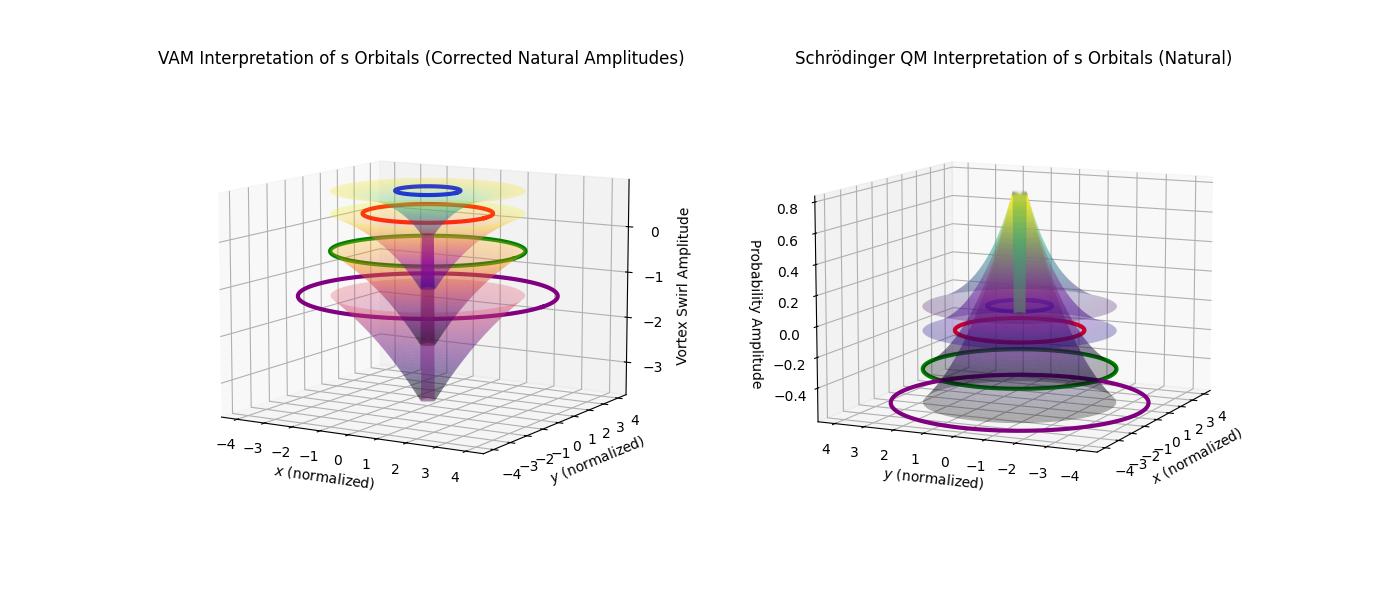
\includegraphics[width=0.7\textwidth]{vortex_diagram}
        \caption{Illustration of a vortex filament in \AE ther.}
        \label{fig:vortex}
    \end{figure}


    \section{Gravity as a Vorticity-Induced Pressure Gradient}\label{sec:gravity-as-a-vorticity-induced-pressure-gradient}
    - Gravitational attraction follows naturally from vortex pressure fields.
    - No singularities; replaces the concept of mass curvature with rotational fluid dynamics.

    \section{Electromagnetism as a Vortex Filament Network}\label{sec:electromagnetism-as-a-vortex-filament-network}
    - Reformulation of Maxwell\rq s Equations in terms of vorticity.
    - Magnetic field as a direct consequence of circulating \AE ther flows.

    \section{Experimental Predictions and Feasibility}\label{sec:experimental-predictions-and-feasibility}
    - Using rotating Bose-Einstein condensates (BECs), we predict vortex filaments to exhibit a circulation-dependent frequency shift measurable via phase-contrast imaging~\cite{kleckner2013}.

    - Electromagnetic anomalies predicted for high-vorticity plasmas.
    - Proposed laboratory tests and detection methods~\cite{kleckner2013, vinen2024, podkletnov2007, orlandi2021}.

    \section{Conclusion}\label{sec:conclusion}
    We have outlined a vortex-based approach to gravity and electromagnetism, As shown in Eq. \eqref{eq:vorticity}, the vorticity transport equation governs  The Vortex \AE ther Model offers a new perspective on fundamental forces,
    replacing spacetime curvature with fluid dynamics in an inviscid \AE ther.
    This framework provides a coherent mathematical model with experimentally testable predictions.
    While VAM provides an alternative to spacetime curvature, further work is needed to derive cosmological implications.
    How does VAM handle large-scale structure formation?
    Can it explain galactic rotation curves without dark matter?
    Future research will explore these avenues.


% Table of Physical Constants used in the Vortex \AE ther Model
    \begin{table}[h]
        \centering
        \renewcommand{\arraystretch}{1.2}
        \begin{tabular}{lllc}
            \toprule
            \textbf{Symbol} & \textbf{Value} & \textbf{Unit} & \textbf{Quantity} \\
            \midrule
            $C_e$ & $1.09384563 \times 10^6$ & $\text{m s}^{-1}$ & Vortex-Core Tangential Velocity \\
            $F_c$ & $29.053507$ & $\text{N}$ & Coulomb Force \\
            $r_c$ & $1.40897017 \times 10^{-15}$ & $\text{m}$ & Vortex-Core Radius \\
            $R_e$ & $2.8179403262 \times 10^{-15}$ & $\text{m}$ & Classical Electron Radius \\
            $c$ & $2.99792458 \times 10^8$ & $\text{m s}^{-1}$ & Speed of Light in Vacuum \\
            $\alpha_g$ & $1.7518 \times 10^{-45}$ & - & Gravitational Coupling Constant \\
            $G$ & $6.67430 \times 10^{-11}$ & $\text{m}^3 \text{kg}^{-1} \text{s}^{-2}$ & Newtonian Constant of Gravitation \\
            $h$ & $6.62607015 \times 10^{-34}$ & $\text{J Hz}^{-1}$ & Planck Constant \\
            $\alpha$ & $7.2973525643 \times 10^{-3}$ & - & Fine-Structure Constant \\
            $a_0$ & $5.29177210903 \times 10^{-11}$ & $\text{m}$ & Bohr Radius \\
            $M_e$ & $9.1093837015 \times 10^{-31}$ & $\text{kg}$ & Electron Mass \\
            $M_{\text{proton}}$ & $1.67262192369 \times 10^{-27}$ & $\text{kg}$ & Proton Mass \\
            $M_{\text{neutron}}$ & $1.67492749804 \times 10^{-27}$ & $\text{kg}$ & Neutron Mass \\
            $k_B$ & $1.380649 \times 10^{-23}$ & $\text{J K}^{-1}$ & Boltzmann Constant \\
            $R$ & $8.314462618$ & $\text{J mol}^{-1} \text{K}^{-1}$ & Gas Constant \\
            $\lambda_c$ & $2.42631023867 \times 10^{-12}$ & $\text{m}$ & Electron Compton Wavelength \\
            \bottomrule
        \end{tabular}
        \caption{List of Physical Constants Used in the Vortex \AE ther Model (VAM)}
        \label{tab:vam_constants}
    \end{table}

    \begin{table}[h]
        \centering
        \renewcommand{\arraystretch}{1.3}
        \begin{tabular}{c l}
            \toprule
            Symbol & Description \\
            \midrule
            \( V \) & Mass of liquid in circular motion (Vortex) \\
            \( \Gamma \) & Vortex circulation strength: \( \oint \mathbf{v} \cdot d\mathbf{s} \) \\
            \( \omega \) & Vorticity magnitude \(\nabla \times \mathbf{v} \) \\
            \( \Phi \) & Vorticity-induced potential function, satisfying \( \nabla^2 \Phi = -\omega \). \\
            \( R \) & Characteristic vortex radius, representing the scale of rotation. \\
            \( \lambda \) & Vortex core parameter, related to the characteristic decay length of vorticity. \\
            \( L \) & Rotational vortex core length \\
            \( \Psi \) & Stream function of vortex motion \( \mathbf{v} = \nabla \times \Psi \). \\
            \( \Psi_k \) & Vortex knot function describing topological structures in the \AE ther. \\
            \( \rh\rho_\text{\ae} \) & Local \AE ther density, assumed to be incompressible in the model. \\
            \( P \) & Pressure in the \AE ther model, often governed by Bernoulli-like principles. \\
            \( H \) & Helicity, a measure of the knottedness of vortex tubes: \( H = \int \mathbf{v} \cdot \mathbf{\omega} \, dV \). \\
            \( K \) & Enstrophy, representing rotational energy density: \( K = \frac{1}{2} \int \omega^2 dV \). \\
            \( \mathbf{v} \) & Velocity vector field \\
            \( \mathbf{\Omega} \) & Angular velocity vector \\
            \( \mathbf{A} \) & Vector potential, where \( \mathbf{B} = \nabla \times \mathbf{A} \) in magnetohydrodynamic analogies. \\
            \( \mathbf{J} \) & Vortex current density, defined by \( \mathbf{J} = \nabla \times \omega \). \\
            \bottomrule
        \end{tabular}
        \caption{Glossary of Terms for Incompressible Non-Viscous Liquid \AE ther}
        \label{tab:symbols}
    \end{table}

    \section{Validated VAM Equations}\label{sec:validated-vam-equations}
    \begin{align}
                \begin{equation}
                R_e = \frac{\lambda_c}{2 \pi} \alpha \\\label{eq:equation4}
                \end{equation}
                \begin{equation}
                R_e = \frac{e^2}{4 \pi \varepsilon_0 M_e c^2} \\\label{eq:equation5}
                \end{equation}
                \begin{equation}
                R_e = 2 r_c \\\label{eq:equation6}
                \end{equation}
                \begin{equation}
                R_e =  \alpha^2 a_0 \\\label{eq:equation7}
                \end{equation}
                \begin{equation}
                R_e = \frac{e^2}{4 \pi \varepsilon_c m_c c^2} \\\label{eq:equation9}
                \end{equation}
                \begin{equation}
                R_e = \frac{e^2}{8 \pi \varepsilon_0 F_{\text{max}} r_c} \\\label{eq:equation8}
                \end{equation}
                \begin{equation}
                R_x = N \frac{F_{\max} r_c^2}{M_e Z C_e^2} \\\label{eq:equation10}
                \end{equation}
                \begin{equation}
                e =\frac{\sqrt{16 \pi F_{\max} r_c^2}}{\mu_0 c^2} \\\label{eq:equation11}
                \end{equation}
                \begin{equation}
                e^2 =16 \pi F_{\max} \xi_0 R_e^2 \\\label{eq:equation13}
                \end{equation}
                \begin{equation}
                e =\frac{\sqrt{2 \alpha h}}{\mu_0 c} \\\label{eq:equation12}
                \end{equation}
                \begin{equation}
                e = \frac{\sqrt{4 C_e h}}{\mu_0 c^2} \\\label{eq:equation14}
                \end{equation}
                \begin{equation}
                R^2 = \frac{N F_{\text {max }} r_c}{4 \pi^2 f^2 m_e} \\\label{eq:equation15}
                \end{equation}
                \begin{equation}
                R^2 = \frac{4 \pi F_{\text{max}} r_c^2}{C_e} \frac{1}{8 \pi^2 M_e f_e} \\\label{eq:equation16}
                \end{equation}
                \begin{equation}
                \frac{1}{r_c} = \frac{c^2}{a_0 2 C_e^2}\label{eq:equation17}
                \end{equation}
    \end{align}








        \section{Vorticity in a Simplified "Rigid-Body" Model}\label{sec:vorticity-in-a-simplified-"rigid-body"-model}

        In fluid mechanics, the vorticity $\omega$ is defined as:
        \[ \omega = \nabla \times \mathbf{v} \]
        where $\mathbf{v}$ is the velocity field of the fluid.

        For an idealized rigid-body rotation about the $z$-axis with constant angular velocity $\Omega$, the velocity field at radius $r$ in cylindrical coordinates is:
        \[ v_{\theta} = \Omega r \]
        A standard result is that the corresponding vorticity magnitude is:
        \[ \omega = 2 \Omega \]
        Thus, the local vorticity is:
        \[ \omega = 2 \frac{v_{\theta}}{r} \]
        which is twice the angular velocity.


        \section{Derivation of the Density of the \AE ther ($\rho_\text{\AE}$)}\label{sec:derivation-of-the-density-of-the-ae{}ther-($rho_text{ae}$)}

        The energy density of a vorticity field is given by:
        \[ E = \frac{1}{2} \rho |\mathbf{\omega}|^2 \]
        where $E$ is the energy density, $\rho$ is the mass density of the \AE{}ther medium, and $\mathbf{\omega}$ is the vorticity field.

        By integrating field interactions across multiple scales, from atomic to cosmological structures, we refine our constraints on $\rho_\text{\AE}$:
        \[ \rho_\text{\AE} \approx 10^{-7} \text{ to } 10^{-5} \text{ kg/m}^3 \]


        \section{Vortex Energy and Swirl Potential}\label{sec:vortex-energy-and-swirl-potential}

        To describe gravitational-like effects in VAM, we introduce the swirl energy potential:
        \[ \Phi_s = \frac{C_e^2}{2F_{\text{max}}} \mathbf{\omega} \cdot \mathbf{r} \]
        where $C_e$ is the core tangential velocity and $F_{\text{max}}$ is the maximum force in the \AE{}theric framework.

        The equivalent expression for gravitational time dilation in VAM is:
        \[ d\tau = \frac{dt}{\sqrt{1 - \frac{C_e^2}{c^2} e^{-r/r_c} - \frac{\Omega^2}{c^2} e^{-r/r_c}}} \]
        where $r_c$ is the vortex core radius and $c$ is the speed of light.


        \section{Experimental Considerations and Predictions}\label{sec:experimental-considerations-and-predictions}

        \subsection{Levitation Effects}\label{subsec:levitation-effects}
        VAM predicts that levitation and lift systems could be optimized by controlling structured resonance fields. The lift force scales as:
        \[ F_L \propto \rho_\text{\AE} \cdot A \]
        where $A$ is the platform area.

        \subsection{Cosmological Energy Density}\label{subsec:cosmological-energy-density}
        Using constraints from vacuum energy studies:
        \[ \rho_\text{vac} \approx 10^{-29} \text{ g/cm}^3 \]
        which, when scaled within the VAM framework, refines \AE{}ther density predictions.


        \section{Conclusion}\label{sec:conclusion2}

        By refining constraints from quantum vortex physics, gravitomagnetic frame-dragging, and cosmological observations, we achieve an improved range of $\rho_\text{\AE}$:
        \[ \rho_\text{\AE} \approx 10^{-7} \text{ to } 10^{-5} \text{ kg/m}^3 \]
        Further experimental and observational studies will help verify these predictions, potentially leading to an even more precise estimate.



    \bibliographystyle{ieeetr}
    \bibliography{references}

\end{document}